\documentclass[oneside,12pt]{discsthesis}
\usepackage{graphicx}
\usepackage{float}
\usepackage{textcomp}
\usepackage{gensymb}
\usepackage{listings}
\usepackage{tabularx}
\usepackage{multirow}
\usepackage{array}
\usepackage[titletoc]{appendix}
\usepackage{textcomp}
\usepackage[normalem]{ulem}
\usepackage[justification=centering]{caption}

\useunder{\uline}{\ul}{}

\newcolumntype{L}{>{\centering\arraybackslash}m{7.5cm}}

\newcolumntype{M}{>{\centering\arraybackslash}m{3cm}}

\newcolumntype{S}{>{\centering\arraybackslash}m{3.5cm}}


\graphicspath{ {Appendices/} }
\begin{document}

 \ThesisAuthor{\textbf{Kennedy E. Espina}}
  \ThesisTitle{\textbf{MULTIDIMENSIONAL SPATIO-TEMPORAL MODELING OF \\ COMMUNICABLE DISEASES USING TWITTER POSTS \\AND HEALTH REPORTS: VISUALIZATION, \\ CORRELATIONS, AND PREDICTION}}
  \ThesisArea{Computer Science}
  \ThesisDefenseYear{2015}
%  \DefenseDate{10 July 2013}
  %\ThesisGrade{Very Good}
  \ThesisStyle{MS}{draft}{-10pt}{15pt}
  % {-10pt}{15pt}

  \FrontMatter

\begin{thesisabstract}

Infodemiology is a relatively new field of study where the margin for innovation is still large. Using infodemiology, the aim of the paper is to determine whether \textbf{tweets} can be an indicator if there is a disease outbreak within a certain area in the Philippines. Different methodologies will be used to get to the result. This includes data extraction, analytics, modeling, and visualization. The modeling of the diseases will be primarily made using IBM's Spatio-Temporal Epidemiological Modeler (STEM). Once a model and a scenario is created in STEM, a simulation of possible disease outbreak locations will be shown on a map based on user-specified timeframe. The results of this research will be especially helpful to the Philippines' Department of Health, as this study complements already existing surveillance system.

\end{thesisabstract}
\tableofcontents
\listoffigures

\MainMatter
 \chapter{Introduction}


Doctors, nurses, and other healthcare practitioners have to deal with huge amounts of information whenever they engage with their work, from pinpointing the various symptoms of a disease to assessing the condition of a patient. Traditionally, patient information is noted down by hand on paper and then collated into folders. This method can get extremely disorganized, with information piling up after years and years; it can also be inconvenient and susceptible to loss, as usually no other copy is made.

The discipline of medical informatics was developed due to the increasing need for a better handling of medical information, as access to healthcare broadens and healthcare institutions grow in size. Patients also have a greater demand for transparency and desire to play a more proactive role with regards to their health. Technology thus comes into play. The current thrust of medical informatics involves developing desktop or mobile applications that give access to databases of patient data. Physical records now become electronic medical records (EMR), so that data such as a patient’s weight or what his treatment was for which appointment can be accessed with a click or a swipe of the finger. This focuses on the patient-specific type of information in medical informatics. The other type is knowledge-based, which is science-oriented rather than people-oriented--for example, an AI that can specify the likely disease as long as one can input the symptoms displayed by the patient \cite{williamr.hersh2002}.

This research is centered on patient-specific information, as it aims to improve on ShineOS+, a mobile and desktop health informatics application that is meant to be used by nurses, doctors, administrators, and other healthcare practitioners as well as patients. Aside from saving patient data, it also has several other features such as keeping track of consultations and appointments, generating reports required by the Department of Health, and streamlining referrals so EMRs can be passed easily from one doctor to another without loss of information. This has immense benefits, some of which may not be as obvious: having the exact prescription noted down digitally can help patients monitor their intake better, and nurses can input their notes so patient profiling becomes more well-rounded. Its use can even be taken beyond the hospital to a disaster setting, where rapid medical help is most needed but where confusion and chaos pose huge obstacles.

One of the strengths of the application is its flexibility--not only is it meant to be used in every digital platform, from Mac OS to Windows to Android, but it also caters to a wide array of users and adapts accordingly. The emphasis is on improving the workflow of the health community, which is one of the major challenges in health informatics, as doctors and nurses can find it difficult and time-consuming to integrate using an app while dealing with patients. Aside from creating an organized system that can present information clearly and thoroughly, the other side of the equation must also be considered: how to design user experience so that users will feel comfortable using it? To a certain extent, this has already been addressed by ShineOS+, as it also allows synchronization between multiple devices and its code is open-source so as to allow innovation and constant responsiveness to the needs of its users. A core tenet of its philosophy is user-centric design, and this seems to have been implemented--a layperson can easily use the app without getting confused and the design is colorful and pleasing.

However, the mobile version--which is still in beta--presents some problems that weren’t present in desktop, which was the original platform. Mobile users are less inclined to fill up long forms. The sheer amount of information presented in one view of the desktop app can become overwhelming when transferred onto mobile. It is very likely, then, that users would not interact significantly with the mobile app because of inconvenience and frustration. This is a significant problem. Phones are much more accessible than laptops, and healthcare practitioners especially need to have the option of being able to enter and access data on the go. Additionally, part of the vision for the application involves turning over more control to the user--custom forms and themes, custom displays, and so on. These have not been implemented yet, and would go a long way towards engaging users.

A possible solution to this problem would be gamification, where game concepts such as reward systems and statistics tracking are applied to a non-game setting in order to make it more compelling to users. This has been successfully used in a wide variety of contexts. A very common example is how customers are given a card so they can rack up points whenever they make a purchase; once they amass enough points, they get a freebie. A website called FreeRice has been quite successful: users answer a trivia quiz, and for every correct answer, the website donates ten grains of rice, as provided by sponsors. Aside from the short-term satisfaction of getting the answer, users also gain a more profound sense of pleasure from being altruistic, and this entices them to return to the website again and again. The most apparent tool used in gamification is giving out rewards. However, relying on this too much can result in an unhealthy infinite loop where the user craves more and more rewards. A more long-term approach would be what is called meaningful gamification, which includes elements such as play (having fun and not being paralyzed by the fear of failure), reflection (connecting the current setting with previous experience or being led to gain insight), and engagement (facilitating an easier and more natural connection between users. Ideally, a sense of narrative is also employed so the user feels as if she is on a quest or a journey \cite{scottnicholson2014}. The challenge faced by this research is, in essence, applying gamification effectively to medical informatics, more specifically through ShineOS+ mobile.

The challenge faced by this research is, in essence, applying gamification effectively to medical informatics, more specifically through ShineOS+ mobile.

\section{Research Questions}

This research aims to answer the question ``How can gamification theory be applied to ShineOS+, an electronic medical record application, to incentivize healthcare practitioners to use the application regularly?''

Other subquestions are as follows:
\begin{itemize}
\item What specific gaming elements can it include to encourage users to use the application?
\item How significant is the change of user engagement and user satisfaction after gamification is applied to the application?

\end{itemize}

\section{Research Objectives}

This research aims to make ShineOS+, a medical informatics mobile app, more appealing and engaging to users through gamification, so that it can fulfill its vision of enhancing the workflow of healthcare practitioners. Examples of gamification might be incorporating reward systems, eliciting a greater sense of community, or giving the user mote autonomy by allowing him greater control over the display (e.g. customizable UI). These modifications will be applied to the app, the new version of which should ready for release by the end of this research.

\section{Scope and Limitations}

As ShineOS+ has a desktop and mobile version, the research would cover applying gamification of the application to both versions. The study will generally focus on enriching the overall user experience by introducing gaming mechanics to reward users for completing tasks listed in the app. In events the app has missing features that would potentially enrich the overall user experience, the research would also cover adding extra functionality to the existing application.
After the implementation of gamification, the study will also analyze if there was a significant improvement in user engagement and user satisfaction.

One of the limitations of this research is that it will not deal with the acquisition of non-virtual rewards, which essentially requires making a deal with pharmaceutical companies. Overall, the research would only limit itself in creating an overall better user experience of the existing application.

\section{Significance of the Study}

Should the gamification prove to be successful, ShineOS+ would extend its user reach and compel more healthcare practitioners to transfer their data onto electronic medical records, especially as this practice is uncommon in the Philippines. This would also make collaboration easier since patient information can be passed from one account to another. Aside from the obvious impact of ease of workflow and a more organized system, long-term use--which is to be encouraged by gamification--might also change the outlook of practitioners on data-keeping. By being able to input the data easily on their phone, they might get into the habit of being more meticulous with checking their patients and jotting down their observations. Transparency would also be encouraged. When the patient asks for an explanation, the practitioner will be able to show the patient’s personalized record from previous consultations, which would lead to them having a more open and informed exchange.

Because electronic medical records are not yet the norm and practitioners may feel reluctant to try them, preferring to stick with the familiar, gamification would provide a bridge. Applying gamification to the mobile version of ShineOS+ can easily be carried over to the desktop version--to the whole cross-platform system, in fact, even MyShine, the corresponding app for patients that is still under development. Instead of seeing record-keeping as a chore, users would come to find it fun and even interesting and would eventually engage in it for their own reasons.

The application of gamification to an electronic medical record application is also a novel idea. While gamification has been applied to various contexts, medical informatics technology tends to be austere, putting most of its focus on the functionality; combining gamification and medical informatics should thus yield interesting results, as they are not commonly put together, and would lead to a more profound understanding, if not new insights, about gamification itself. Rather than short-term change, what this research aims for is for users to consult ShineOS+ regularly--to have it become an integral part of their everyday workflow--which only high-level gamification would achieve.


 \chapter{Review of Related Literature}

This research concerns itself in gamification of a medical informatics application to keep the user engaged and promote the use of Shine OS+. The review of related literature is divided into two sections and proceeds as follows: \textbf{Gamification Theories and its Applications} and \textbf{Medical Informatics}.

\section{Gamification}

Kapp defines gamification as “Using game-based mechanics, aesthetics and game thinking to engage people, motivate action, promote learning, and solve problems”. There are many definitions of gamification but the one that is always similar is that it is a tool to “increase engagement in some activity using game features, providing enjoyment and fun”, the use of game elements in non-gaming systems to improve user experience and user engagement \cite{karlmkapp2012}. Unsurprisingly, there has been a growing trend of the use of gamification to capture the target audience of traditional applications \cite{luisRodrigues2016}. One of the benefits that gamification brings is the promise of new design patterns and a more interactive user experience. With the interests of businesses to keep users engaged and entertained in using the app for as long as possible, it is not surprising that we have seen the application of game mechanics of many non game related contexts.

In gamification, the focus is not the game itself but they have a significant role as a motivation tool for users to continue using the app \cite{alidarejeh2016}. Gamification has seen a wide array of applications in different disciplines. Ali Darejeh and Siti Salwah Salim lists down the most common contexts of the usage of gamification:
\begin{itemize}
\item Human Resources. Many applications have proven to be successful to increase personnel motivation, engagement and working performace.
\item Health care and Sport. With the help of gamification, people have shown an increase of desire to do physical activities, which promotes to live healthy and motivate hospital patients to continue taking their medicines.
\item E-Learning. Gaming in education helps students to spend more time in learning the reading material and increase their class activity by asking and answering questions in the systems.
\item Data Collection. Gamification motivates people to participate in the collection of data, such as getting crowdsourced information for research.
\item Online Community. Gamification encourages users to to participate in a certain online community such as blogs, social websites and others.
\item Software Popularity. Lastly, gamification increase the loyalty of customers to use specific products for a long time. This also translates to an increased frequency of using the software and a discovery-based learning.
\end{itemize}

There are many examples of gamification that can be seen in present mobile applications such as Endomondo, Nike Plus and FourSquare \cite{alidarejeh2016}. In Endomondo and Nike Plus, they make use of special badges and points when they run a certain distance or participate in a predefined activity listed in the app. Similarly in Foursquare, users receive badges when they visit a special place and use the app to check-in. The use of virtual badges and points are to make the users more motivated, and to continuously encourage the use of the app. Most apps also make use of leaderboards to add a social dimension and a sense of competition among its users.

\subsection{Self Determination Theory}

The theory behind the motivation of users when using a gamified application is usually the SDT (Self Determination Theory) \cite{karlmkapp2012}. The theory states that the human being has three basic needs: competence, relatedness, and autonomy. A person is motivated to perform a certain activity based on the level of these three needs \cite{andrade2016bright}. The theory further suggests that the degree of motivation can vary from amotivation, without any motivation at all to perform an activity, to intrinsic motivation, when the user does not need any external incentives to perform the activity \cite{karlmkapp2012}. The gamification theory then proposes that the use of gaming elements in any application will be able to satisfy some of the users’ basic needs which would make the activity more attractive, even though the user is not intrinsically motivated.

As seen in many gamified apps, gamification is commonly associated with adding a scoring system in order to motivate users--badges, proof of status, points, and so on. While this may work out successfully in the short term, this may have a detrimental effect over the long-term. Scoring systems function as rewards that give users external motivation. Psychological studies have found that people respond immediately to rewards and external motivation can easily be provided. However, external motivation has an inverse relationship to internal motivation, wherein the user continues engaging in an activity because of an innate desire to; he would do it even without a reward \cite{reeve2004}.

An example of rewards decreasing internal motivation can be found in the school setting. Students’ work are graded by teachers, and these grades supposedly function as feedback on how they are doing. While this can motivate students to improve their performance, students also tend to cease to put effort when they realize that they will not be graded. This shows the pitfall of targeting users through rewards: they have to keep receiving rewards, or else engagement will drop altogether. Reffered to as reward gamification, and among the criticisms thrown at it is that it is hardly “gamelike” at all, as the most prominent game element it borrows is the scoring system and this is the least interesting part \cite{nicholson2012user}.

\subsection{Meaningful Gamification}

In order to propose an alternative model that is less exploitative of users and that has a greater possibility of sparking long-term change, an alternative view is the organismic integration theory. Organismic Integration Theory, which studies how external rewards can be internalized and integrated into one’s sense of self, states that users fare better when the activity somehow becomes aligned with their personal goals and connected with their values. In comparison, users motivated by external controls will have a more negative perception of the activity \cite{reeve2004}.
Another theory is Universal design for Learning. Courses should adapt to different learners \cite{rose2000universal}. When transferred to a gamification context, this means that either users should be allowed to make their own goals or there should be different ways for them to reach these goals. A scoreboard may appeal to the competitiveness in some users, but other users might have a different way of assessing how much they’ve achieved and thus would not find this meaningful \cite{nicholson2012user}.

Ultimately, Nicholson is putting forward a model that he calls meaningful gamification, where the user is driven by intrinsic rather than extrinsic motivation. The user must thus be at the center. Rather than asking about what benefits the organization would like to have, the designer of the application ought to be concerned first about how to help the user. In this way, the benefits become mutual: users become engaged in and derive value from the application, which of course would have a positive turnout for the organization \cite{nicholson2012user}.

However, this is not meant to discredit using reward systems altogether, as they still have their use when it comes to getting immediate responses from the user. In very specific situations, they can also pave the way for long-term change. When getting the user to learn a real-world skill, such as programming or cooking, doling out rewards could work. As the user progresses, he might eventually realize the significance of learning such a skill and derive intrinsic satisfaction without the need for external rewards anymore. This is why the recommended approach is to bring users in using a light reward system initially, then once their attention is sufficiently captured, this can be replaced by meaningful gamification \cite{scottnicholson2014}.

As for what constitutes meaningful gamification, Nicholson lists down six elements taken from game design: play, exposition, choice, information, engagement, and reflection.
\begin{itemize}
\item Play is almost always synonymous with fun; the user must participate in it by her own choice, and she should be given ample freedom to explore and make mistakes. The difference between play and a game is that “a game is a form of play with goals and structures \cite{maroneykevin2001}.” A gamified system must thus allow the users to create their own rules and change them when necessary--temporary rules, in other words.
\item Exposition refers to embedding a narrative in the system. The user can see herself as being part of a storyline, journey, or quest, which provides continuity through time and gives a sense of progress and growth. This is an especially powerful tool because human beings naturally process everything in terms of narrative.
\item If a set narrative is to be provided rather than giving the user free reign to create his own, which can be difficult to implement in technological systems, then this has to be balanced with the user’s autonomy or freedom of choice. The more that a user can customize an application, or the more tailor-fitted it is to him rather than being generic, the more involved the user feels, and the greater his sense of positive wellbeing.
\item Next is information. Rather than stopping short at being showered with points, users must also know how and why they are being rewarded. An example of this element in an actual game is the wise sage that guides the player by giving her knowledge. This caters to the user’s need for mastery, which is one of the components of intrinsic motivation.
\item Engagement can refer to either: (1) capturing the user’s interest and getting him into a state of flow; or (2) getting her to connect with others. Flow occurs when one becomes so absorbed in doing an activity that one loses track of time. This happens when an activity pushes the user out of her comfort zone, but at a level that she can handle, which leads the user to improvement. As she grows, the level of difficulty that she needs in order to experience flow also rises. If the level is kept too easy and no opportunity for growth is provided, the user lapses off into boredom \cite{mihalycsikszentmihalyi2008}. On the other hand, the social aspect of engagement is based on the user’s feeling of connection with other people, commonly expressed in applications through social networks and peer-to-peer exchanges. Avenues of social engagement can be chat boards and forums; they can also have a competitive slant, such as scoring systems or users playing against each other.
\item Finally, reflection means that the user can find a significant connection between the system and his life experiences. Without this, it would be impossible to find meaning in the system or to engage in it meaningfully. The process of reflection starts with a direct experience; the user then relates this experience with his life, then makes generalized conclusions based on this, and applies this to a whole set of new experiences as the cycle starts all over again \cite{kolb1981learning}. Through reflection, the user can take what he learned from the system and actually carry it over to the real world.
\end{itemize}

Aside from letting rewards-based transition to meaningful gamification, the gamification must also be designed to end; it should not be kept up indefinitely, as this will make the user dependent. Ideally, gamification should leave the user more equipped to deal with the real world: the application should instill long-term change in the user. As Nicholson points out, \enquote{the goal of the journey is to remove the gamification layers entirely... Gamification should not be thought of as a cycle, but as a journey to bring about lifelong change} \cite{scottnicholson2014}.

\section{General Success of Medical Informatics}

Health information technology is a relatively new field that has been gaining traction over the past few decades, and an aspect of it that has received much attention is EMR (electronic medical records), wherein patient data are stored digitally rather than written down on paper (reference). While the benefits are clear -- healthcare workflow becomes efficient and resources are maximized -- the problem lies in how to connect with users. Functional systems are developed, but users do not adapt well to these -- in fact, almost 45\% of these systems are abandoned. What is more alarming is that 85\% become ultimately ineffective, and only 15\% are successful. Instead of focusing only on tne technology, the context -- the people and organizations involved -- must also be understood as thoroughly as possible \cite{premji2012implementing}.

\subsection{Medical Informatics in the Philippines}

Health information technology is already being used extensively in Asian countries such as Singapore. Computers play an essential role in the hospitals of nearly all Asian countries, but what kind of systems are involved and how well they are used varies from country to country, with a certain dependence on the government and how much budget it is willing to allocate \cite{nguyen2008analysis}. Implementation in Europe and USA are still fraught with issues as well, as there is no one-size-fits-all system, but it is even trickier in developing countries, where health crises are prevalent (e.g. AIDS and malaria), and infrastructure and staff are lacking \cite{fraser2005implementing}.

In the Philippines, medical informatics was already present since the 1980s. The most basic form of this was residents inputting patient information into IBM-compatible machines. Development proceeded more quickly in the 1990s, when the University of the Philippines Manila opened a Medical Informatics Unit composed of academics. They engaged in extensive research, but no concrete, long-standing projects were built that would involve the public. However, they did shape local medical informatics to be distinct from what is practiced in other countries by making it community-focused. In contrast to first-world countries, which have sophisticated facilities, the UP College of Medicine consistently put the community at the forefront \cite{marcelo2007health}. e-Health Philippines was also started in 1998 in order to make it more appealing for researchers to create specialty databases \cite{nguyen2008analysis}.

\subsection{Challenges in Philippines' Medical Informatics}

As of now, like other Southeast Asian countries, there have been several attempts to make medical informatics an integral part of Philippine healthcare, but these have not been as successful as hoped for because of several factors \cite{nguyen2008analysis}:.

\begin{enumerate}
    \item Lack of interest in people

    A major stumbling block is sparking the sustained interest of healthcare professionals and decision-makers such as government officials. Some of them do not realize the immense benefits that medical informatics could provide. Those who wanted to try it seemed to be motivated only by the desire for novelty and stopped using it after a while \cite{marcelo2007health},  and the number of doctors is decreasing because many of them are switching to nursing careers so they can migrate abroad \cite{nguyen2008analysis}.

    Healthcare providers can also be reluctant to embrace new technology, especially those belonging to the older generation, as they are already comfortable with the paper-based system. They may also have never used computers before and may be anxious or fearful ("I have a computer at home but I don't really turn it on because I'm scared it might explode.") \cite{premji2012implementing}. However, they acknowledge that the paper-system can be tiring and tedious, and they tend to compromise the quality of their service because there is too much paperwork for them to do.
    \item Lack of funds

    The Department of Health, as the primary local agency in charge of health, releassd Formula One for Health in 2005, which aims to reform the local health sector. There is a notable focus on finances, as the DOH planned to make the spending of public funds more transparent in order to secure more support for the health sector. In the Philippines, the health sector can be divided into two: public and private. It is unique among Southeast Asian countries because most of its medical services come from the private sector. The percentage of money allocated by the government into healthcare is already low and steadily decreasing every year, so the public sector caters more to patients who lack the money to go to private hospitals \cite{nguyen2008analysis}.
    \item Lack of decentralization

    The health sector is also far from being decentralized, with great reliance on central rather than peripheral authorities. Data are gathered locally, then passed on step by step to organizations until they reach DOH; DOH then comes up with health policies based on these data, and these flow back down. This setup is inefficient and ineffective. The World Health Organizafion (WHO) suggested at the 1978 conference at Alma-Ata that district health systems would benefit from decentralization. Two attempts were made to reform the system in the Philippines, in 1991 and 1998, but these failed because they chose to keep recording data on paper.

    In any endeavor to promote medical informatics, the DOH is a major influencer from a larger perspective, as shown by centralization: it inevitably influences decision-making because it is in charge of the report submission process. Local government units also have to be taken into account. If their support is not obtained or if tension exists, then it is unlikely that a system would be successful \cite{premji2012implementing}.
    \item Network Infrastructure

    Technology has become increasingly cheap, with most developing countries having easy access to internet \cite{fraser2005implementing}. However, not everyone in the Philippines is comfortable with computers, much less even own them; phones are more prevalent, but these may not be able to download complex applications. Moreover, several remote areas, where health workers are needed, do not have electricity \cite{marcelo2007health}. If a system is to be built, then all the available resources must be accounted for, and cost must be weighed against benefits.
\end{enumerate}

\subsection{Case Study: CHITS}

A system called the Community Health Information Tracking System (CHITS) was implemented by the Medical Informatics Unit of UP Manila. This could store electronic health records as well as set clinic appointments, and this was tested out in at least 36 health centers. An observation of their process of introducing the system to its users yields several psychological insights \cite{premji2012implementing}

Healthcare providers as well as government officials were carefully guided through a step-by-step training; when exposed to the technology so that they became comfortable enough with it, they realized how much more efficient and easy it is to use. Those unfamiliar with computers warmed up to it by playing simple games then moving on to more complex tasks \cite{premji2012implementing}.

The learning curve remained steep, however. Every day for the next few months, healthcare providers used the paper-based system during busy hours at work, then practiced the electronic system when they had more time. Some of them still remained anxious, but most of them got past their discomfort and became proficient at it. This gave them a sense of pride about the new skill that they'd mastered. They also experienced immense relief at being able to print everything at the end of the day rather than filling up all the forms by hand. As a result, patients were handled with less delay. As one provider said: " In the manual, paper-based system it [took] 10 minutes to find a patient record but now it takes seconds to find." They also trusted the data more, so when they noticed patterns that hinted at an outbreak, they told the head physician right away \cite{premji2012implementing}.


% Gamification is defined as the use of game elements in non-gaming systems to improve user experience and user engagement. Unsurprisingly, there has been a growing trend of the use of gamification to capture the target audience of traditional applications \cite{luisRodrigues2016}. One of the benefits that gamification brings is the promise of new design patterns and a more interactive user experience. With the interests of businesses to keep users engaged and entertained in using the app for as long as possible, it is not surprising that we have seen the application of game mechanics of many non game related contexts.
%
% As seen in many gamified apps, gamification is commonly associated with adding a scoring system in order to motivate users--badges, proof of status, points, and so on. While this may work out successfully in the short term, this may have a detrimental effect over the long-term. Scoring systems function as rewards that give users external motivation. Psychological studies have found that people respond immediately to rewards and external motivation can easily be provided. However, external motivation has an inverse relationship to internal motivation, wherein the user continues engaging in an activity because of an innate desire to; he would do it even without a reward \cite{reeve2004}.
%
% An example of rewards decreasing internal motivation can be found in the school setting. Students’ work are graded by teachers, and these grades supposedly function as feedback on how they are doing. While this can motivate students to improve their performance, students also tend to cease to put effort when they realize that they will not be graded. This shows the pitfall of targeting users through rewards: they have to keep receiving rewards, or else engagement will drop altogether. Reffered to as reward gamification, and among the criticisms thrown at it is that it is hardly “gamelike” at all, as the most prominent game element it borrows is the scoring system and this is the least interesting part \cite{nicholson2012user}.
%
% In order to propose an alternative model that is less exploitative of users and that has a greater possibility of sparking long-term change, an alternative view is the organismic integration theory. Organismic Integration Theory, which studies how external rewards can be internalized and integrated into one’s sense of self, states that users fare better when the activity somehow becomes aligned with their personal goals and connected with their values. In comparison, users motivated by external controls will have a more negative perception of the activity \cite{reeve2004}.
% Another theory is Universal design for Learning. Courses should adapt to different learners \cite{rose2000universal}. When transferred to a gamification context, this means that either users should be allowed to make their own goals or there should be different ways for them to reach these goals. A scoreboard may appeal to the competitiveness in some users, but other users might have a different way of assessing how much they’ve achieved and thus would not find this meaningful \cite{nicholson2012user}.
%
% Ultimately, Nicholson is putting forward a model that he calls meaningful gamification, where the user is driven by intrinsic rather than extrinsic motivation. The user must thus be at the center. Rather than asking about what benefits the organization would like to have, the designer of the application ought to be concerned first about how to help the user. In this way, the benefits become mutual: users become engaged in and derive value from the application, which of course would have a positive turnout for the organization \cite{nicholson2012user}.
%
% However, this is not meant to discredit using reward systems altogether, as they still have their use when it comes to getting immediate responses from the user. In very specific situations, they can also pave the way for long-term change. When getting the user to learn a real-world skill, such as programming or cooking, doling out rewards could work. As the user progresses, he might eventually realize the significance of learning such a skill and derive intrinsic satisfaction without the need for external rewards anymore. This is why the recommended approach is to bring users in using a light reward system initially, then once their attention is sufficiently captured, this can be replaced by meaningful gamification \cite{scottnicholson2014}.
%
% As for what constitutes meaningful gamification, Nicholson lists down six elements taken from game design: play, exposition, choice, information, engagement, and reflection.
% \begin{itemize}
% \item Play is almost always synonymous with fun; the user must participate in it by her own choice, and she should be given ample freedom to explore and make mistakes. The difference between play and a game is that “a game is a form of play with goals and structures \cite{maroneykevin2001}.” A gamified system must thus allow the users to create their own rules and change them when necessary--temporary rules, in other words.
% \item Exposition refers to embedding a narrative in the system. The user can see herself as being part of a storyline, journey, or quest, which provides continuity through time and gives a sense of progress and growth. This is an especially powerful tool because human beings naturally process everything in terms of narrative.
% \item If a set narrative is to be provided rather than giving the user free reign to create his own, which can be difficult to implement in technological systems, then this has to be balanced with the user’s autonomy or freedom of choice. The more that a user can customize an application, or the more tailor-fitted it is to him rather than being generic, the more involved the user feels, and the greater his sense of positive wellbeing.
% \item Next is information. Rather than stopping short at being showered with points, users must also know how and why they are being rewarded. An example of this element in an actual game is the wise sage that guides the player by giving her knowledge. This caters to the user’s need for mastery, which is one of the components of intrinsic motivation.
% \item Engagement can refer to either: (1) capturing the user’s interest and getting him into a state of flow; or (2) getting her to connect with others. Flow occurs when one becomes so absorbed in doing an activity that one loses track of time. This happens when an activity pushes the user out of her comfort zone, but at a level that she can handle, which leads the user to improvement. As she grows, the level of difficulty that she needs in order to experience flow also rises. If the level is kept too easy and no opportunity for growth is provided, the user lapses off into boredom \cite{mihalycsikszentmihalyi2008}. On the other hand, the social aspect of engagement is based on the user’s feeling of connection with other people, commonly expressed in applications through social networks and peer-to-peer exchanges. Avenues of social engagement can be chat boards and forums; they can also have a competitive slant, such as scoring systems or users playing against each other.
% \item Finally, reflection means that the user can find a significant connection between the system and his life experiences. Without this, it would be impossible to find meaning in the system or to engage in it meaningfully. The process of reflection starts with a direct experience; the user then relates this experience with his life, then makes generalized conclusions based on this, and applies this to a whole set of new experiences as the cycle starts all over again \cite{kolb1981learning}. Through reflection, the user can take what he learned from the system and actually carry it over to the real world.
% \end{itemize}
%
%  Aside from letting rewards-based transition to meaningful gamification, the gamification must also be designed to end; it should not be kept up indefinitely, as this will make the user dependent. Ideally, gamification should leave the user more equipped to deal with the real world: the application should instill long-term change in the user. As Nicholson points out, `'the goal of the journey is to remove the gamification layers entirely... Gamification should not be thought of as a cycle, but as a journey to bring about lifelong change `' \cite{scottnicholson2014}.

 \chapter{Methodology}

The primary focus of this research is the infodemiological surveillance of three (3) of the top communicable diseases - Measles, Influenza, Typhoid Fever -  in the Philippines, as reported by the Philippines' Department of Health (DOH) \cite{dohrecord2015}. The research is divided into two parts, which are 1) collection of health-related tweets and their visualization in a map, and 2) the modeling and prediction of possible areas of outbreaks based on Twitter posts.

This section breaks down the phases further into five (5) subsections, \textit{Health Data Collection}, \textit{Infodemiological Modeling and Classification}, \textit{Twitter Data Visualization}, \textit{Epidemiological Correlation and Modeling}, and \textit{STEM Scenario Visualization}. The overview of the methodology can be seen in Figure \ref{fig:GeneralMethodology}.


\begin{figure}[!ht]
    \centering
    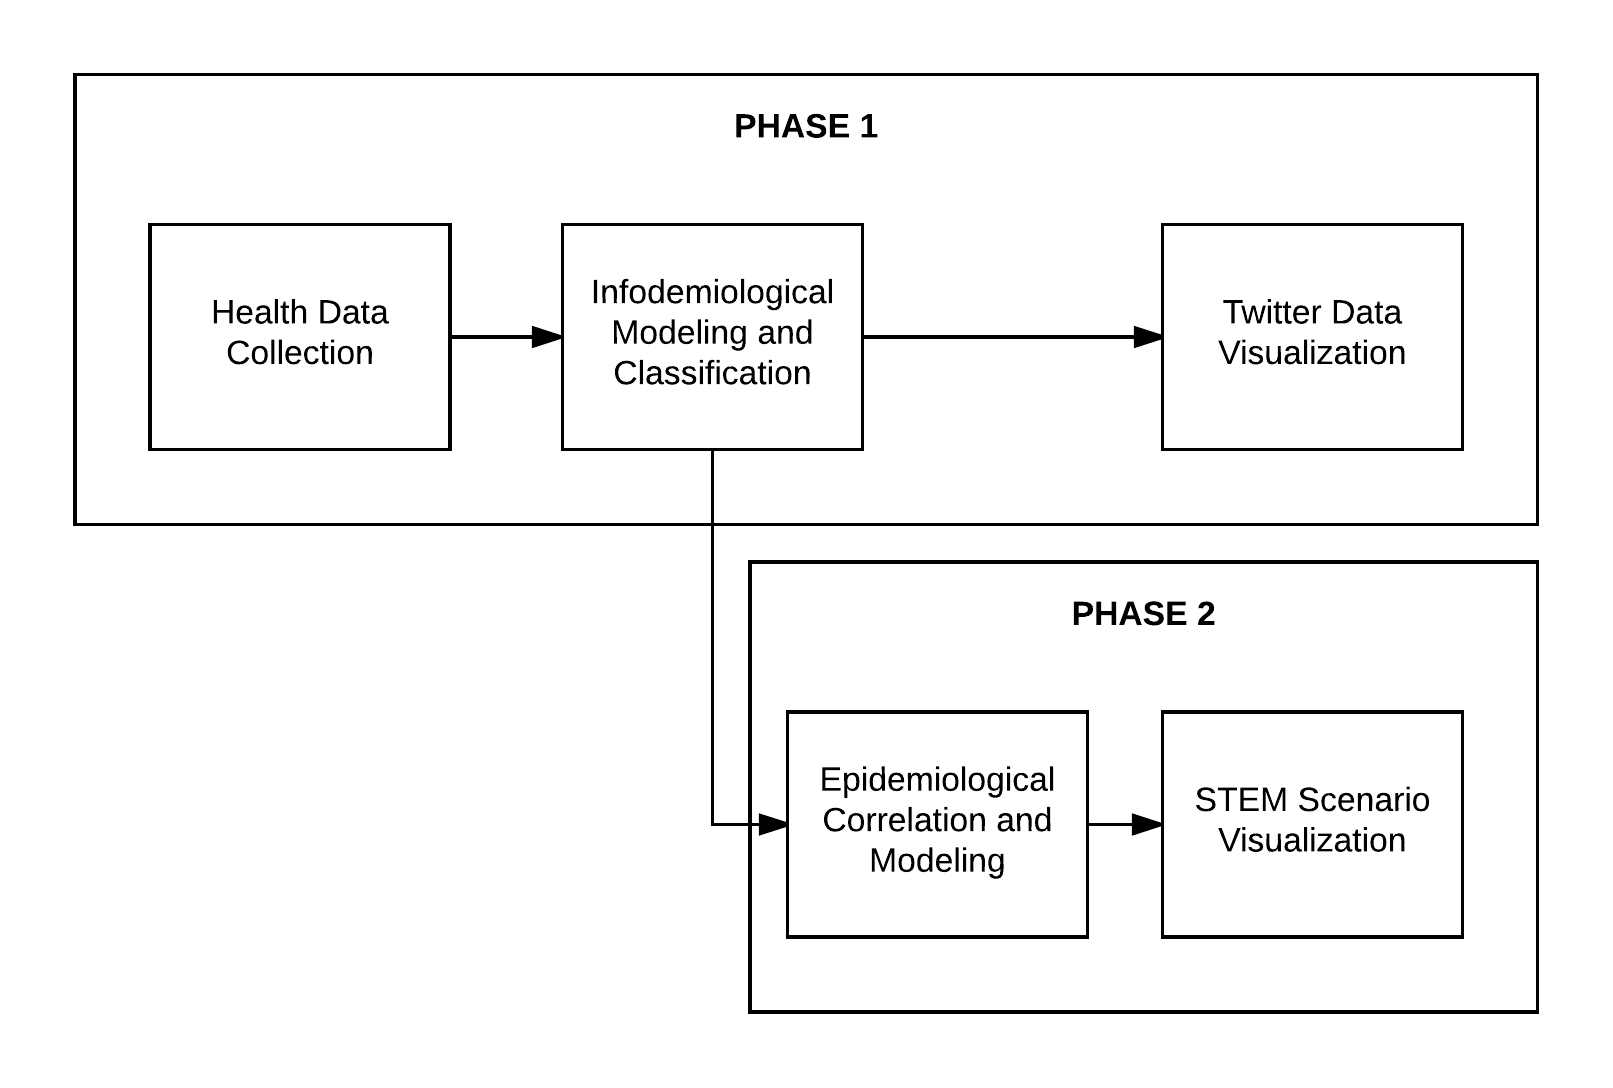
\includegraphics[width=\textwidth]{GeneralMethodology}
	\caption{General view of the research's methodology.}
	\label{fig:GeneralMethodology}
\end{figure}

\section{Health Data Collection}
The data that will be used for the research comes from two (2) sources, which are 1) publicly available individual posts collected from \textbf{Twitter}, which then will be validated through 2) publicly available statistical documents that largely leverages on the data by \textbf{Philippines' Department of Health (DOH)}. The users' posts from Twitter represents majority of the data to be processed, while the supporting records and documents act as a sustained supplementary data to be used as a baseline for comparison, correlation, and prediction.

\subsection{Twitter Data Collection}
Through the use of Twitter's public streaming Advanced Programming Interfaces (API), a tool will be used to gather relevant tweets through using keywords. The tool developed by the Ateneo Java Wireless Competency Center (AJWCC) is the chosen tweet collector that will be used. The tool is based on the \textit{Ruby on Rails} programming language and framework, using the \textit{tweetstream} gem. The tool collects tweets in realtime based on the supplied keywords in its configuration file. It will be deployed on a local server with a constant connection to the Internet. This means that the collection will happen the whole day. The official start of collection for real-time tweet collection will be on \textit{June 13, 2016} until \textit{September 13, 2016}. Added to real-time collection, the research will also be accessing historical tweets through the AJWCC as well.

\subsubsection {Keyword Compilation}
Based on the related literature review, words associated to the disease will be gathered. Listed are possible keyword groups that may be found in social media posts.

\begin{itemize} 
\item \textbf{Coloquial Terms} - Terms used by the people that may indicate the presence of flu.
	\begin{itemize} 
		\item Example: \textit{``lagnat"}, \textit{``flu"}, \textit{``sick"}
	\end{itemize}
\item \textbf{Symptoms} - The symptoms of influenza. This includes both English and Filipino words.
	\begin{itemize} 
		\item Example: \textit{``ubo''}, \textit{``cough''}, \textit{``sipon''}, \textit{``sneeze''}
	\end{itemize}
\item \textbf{Behavior/Actions} - The behavior of people when they have the flu. For example, people  buy medicines during flu seasons, therefore drugstores, in general, may be used as a keyword.
	\begin{itemize} 
		\item Example: \textit{``mercury drug''}, \textit{``stay in bed''}, \textit{``tulog''}, \textit{``gamot''}
	\end{itemize}
\item \textbf{Weather Condition} - Lastly, the weather conditions of an area. Flu seasons arise when it's cold.
\begin{itemize} 
		\item Example: \textit{``rain''}, \textit{``ulan''}, \textit{``cold''}
	\end{itemize}
\end{itemize}

These keywords, along with their conjugations if possible, will be used as the search parameters for Twitter. 

\subsection{Department of Health - Epidemiology Bureau Data}

Regularly, the Philippines' Department of Health publishes through their websites their gathered disease surveillance statistics. This can be accessed by visiting \textit{http://nec.doh.gov.ph/}. Since these data directly come from the DOH, these can be considered as a the gold standard for correlation and regression.

% Besides the published statistics found in the Department of Health's website, through the project headed by Dr. Regina Estuar in cooperation with the DOH's Surveillance in Post Extreme Emergencies and Disasters (SPEED) project \cite{whatisspeed}, data sets can be gathered directly from the department itself to be used in the correlation computation. SPEED is a warning surveillance system used by the DOH after disasters to help in identifying trends in people's health conditions, and ultimately, to help in preventing diseases from spreading \cite{whatisspeed}. Because of the surveillance nature of this project, the data being collected can be considered as an accurate source for correlation with the gathered tweets.


\bibliographystyle{plain}
\bibliography{ResearchBibliography}

\addappheadtotoc
\appendix{Geocoded XML of \textit{``Metro Manila''} using Google Maps Geocode API} \label{App:GeocodeXML}
	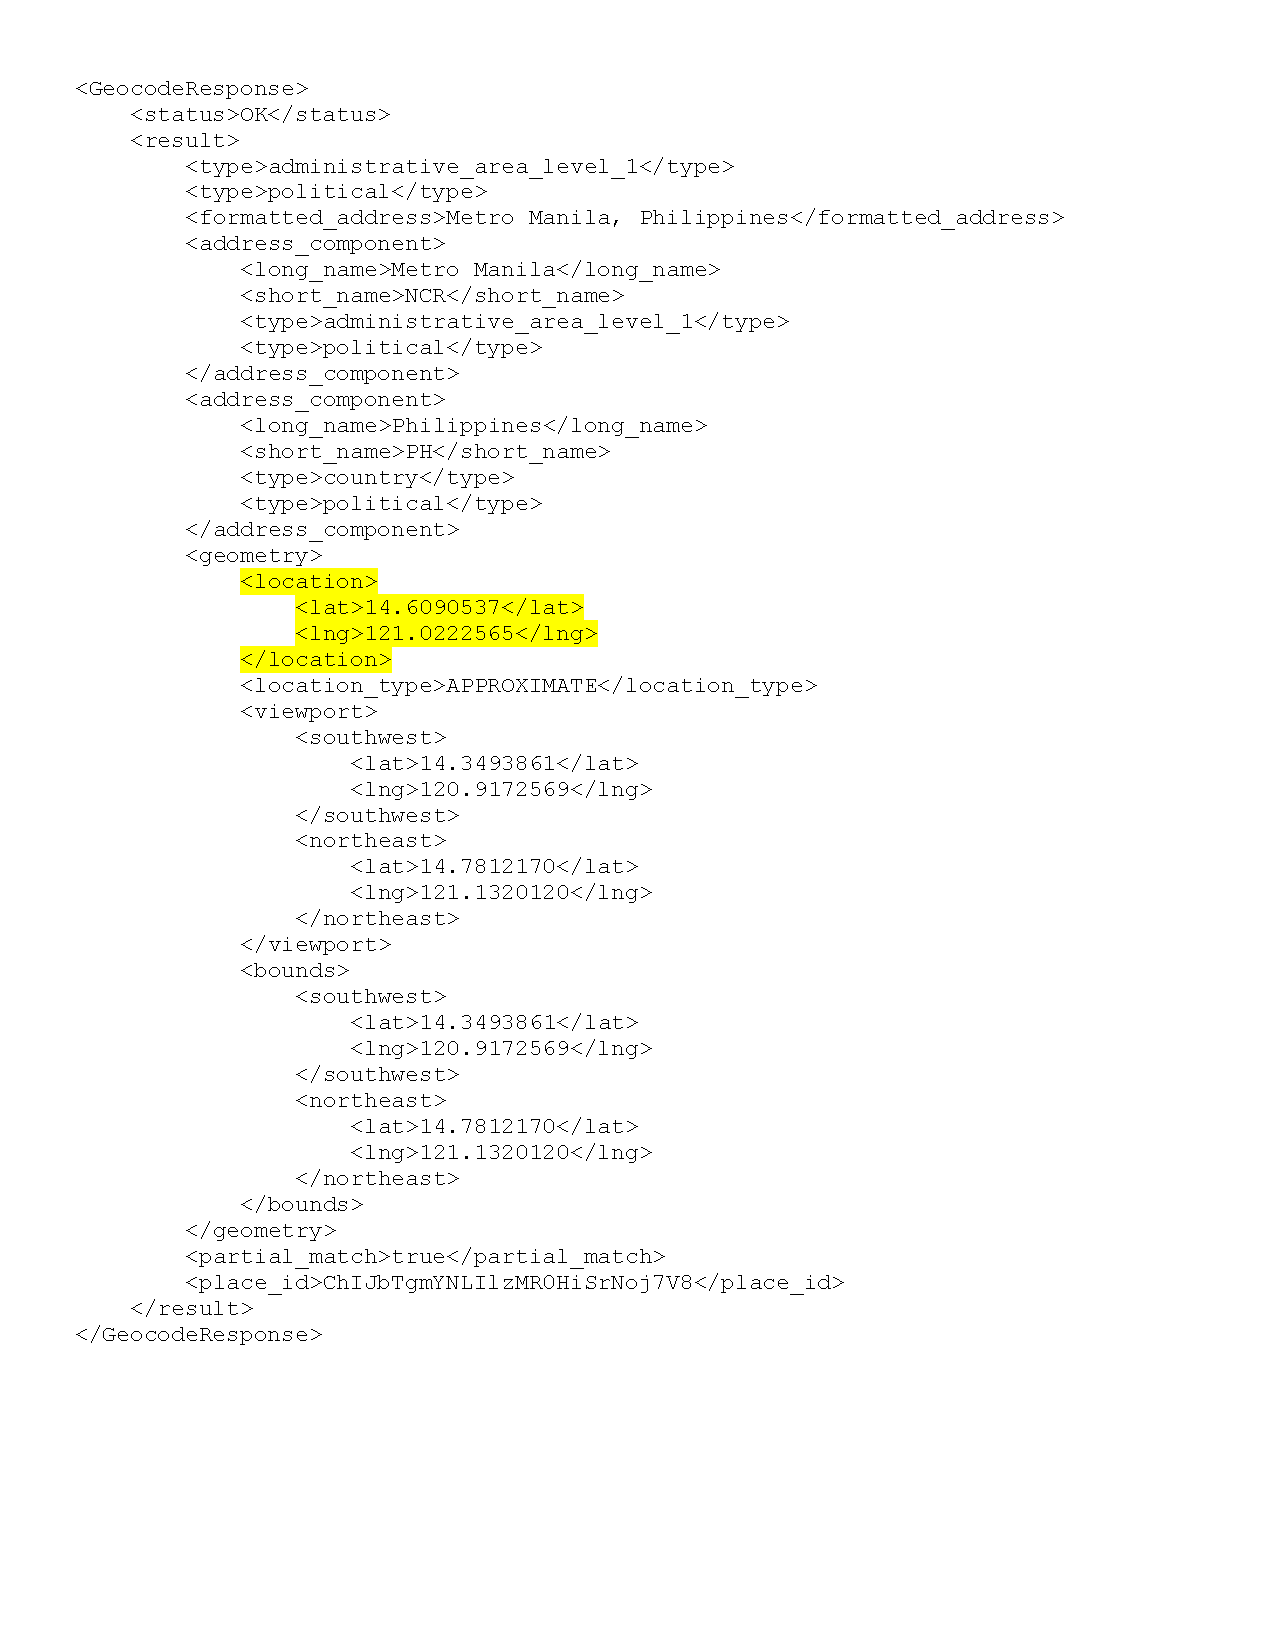
\includegraphics[page=1,width=\textwidth,scale=1]{GeocodeXmlSample.pdf}


\end{document}
